\documentclass{fkssolpub}

\usepackage[czech]{babel}
\usepackage{fontspec}
\usepackage{fkssugar}
\usepackage{amsmath}
\usepackage{graphicx}

\newcommand{\dd}{\mathrm{d}}
\renewcommand{\angle}{\sphericalangle}

\author{Ondřej Sedláček}
\school{Gymnázium Oty Pavla} 
\series{5}
\problem{G} 

\begin{document}

\begin{figure}
  \begin{center}
    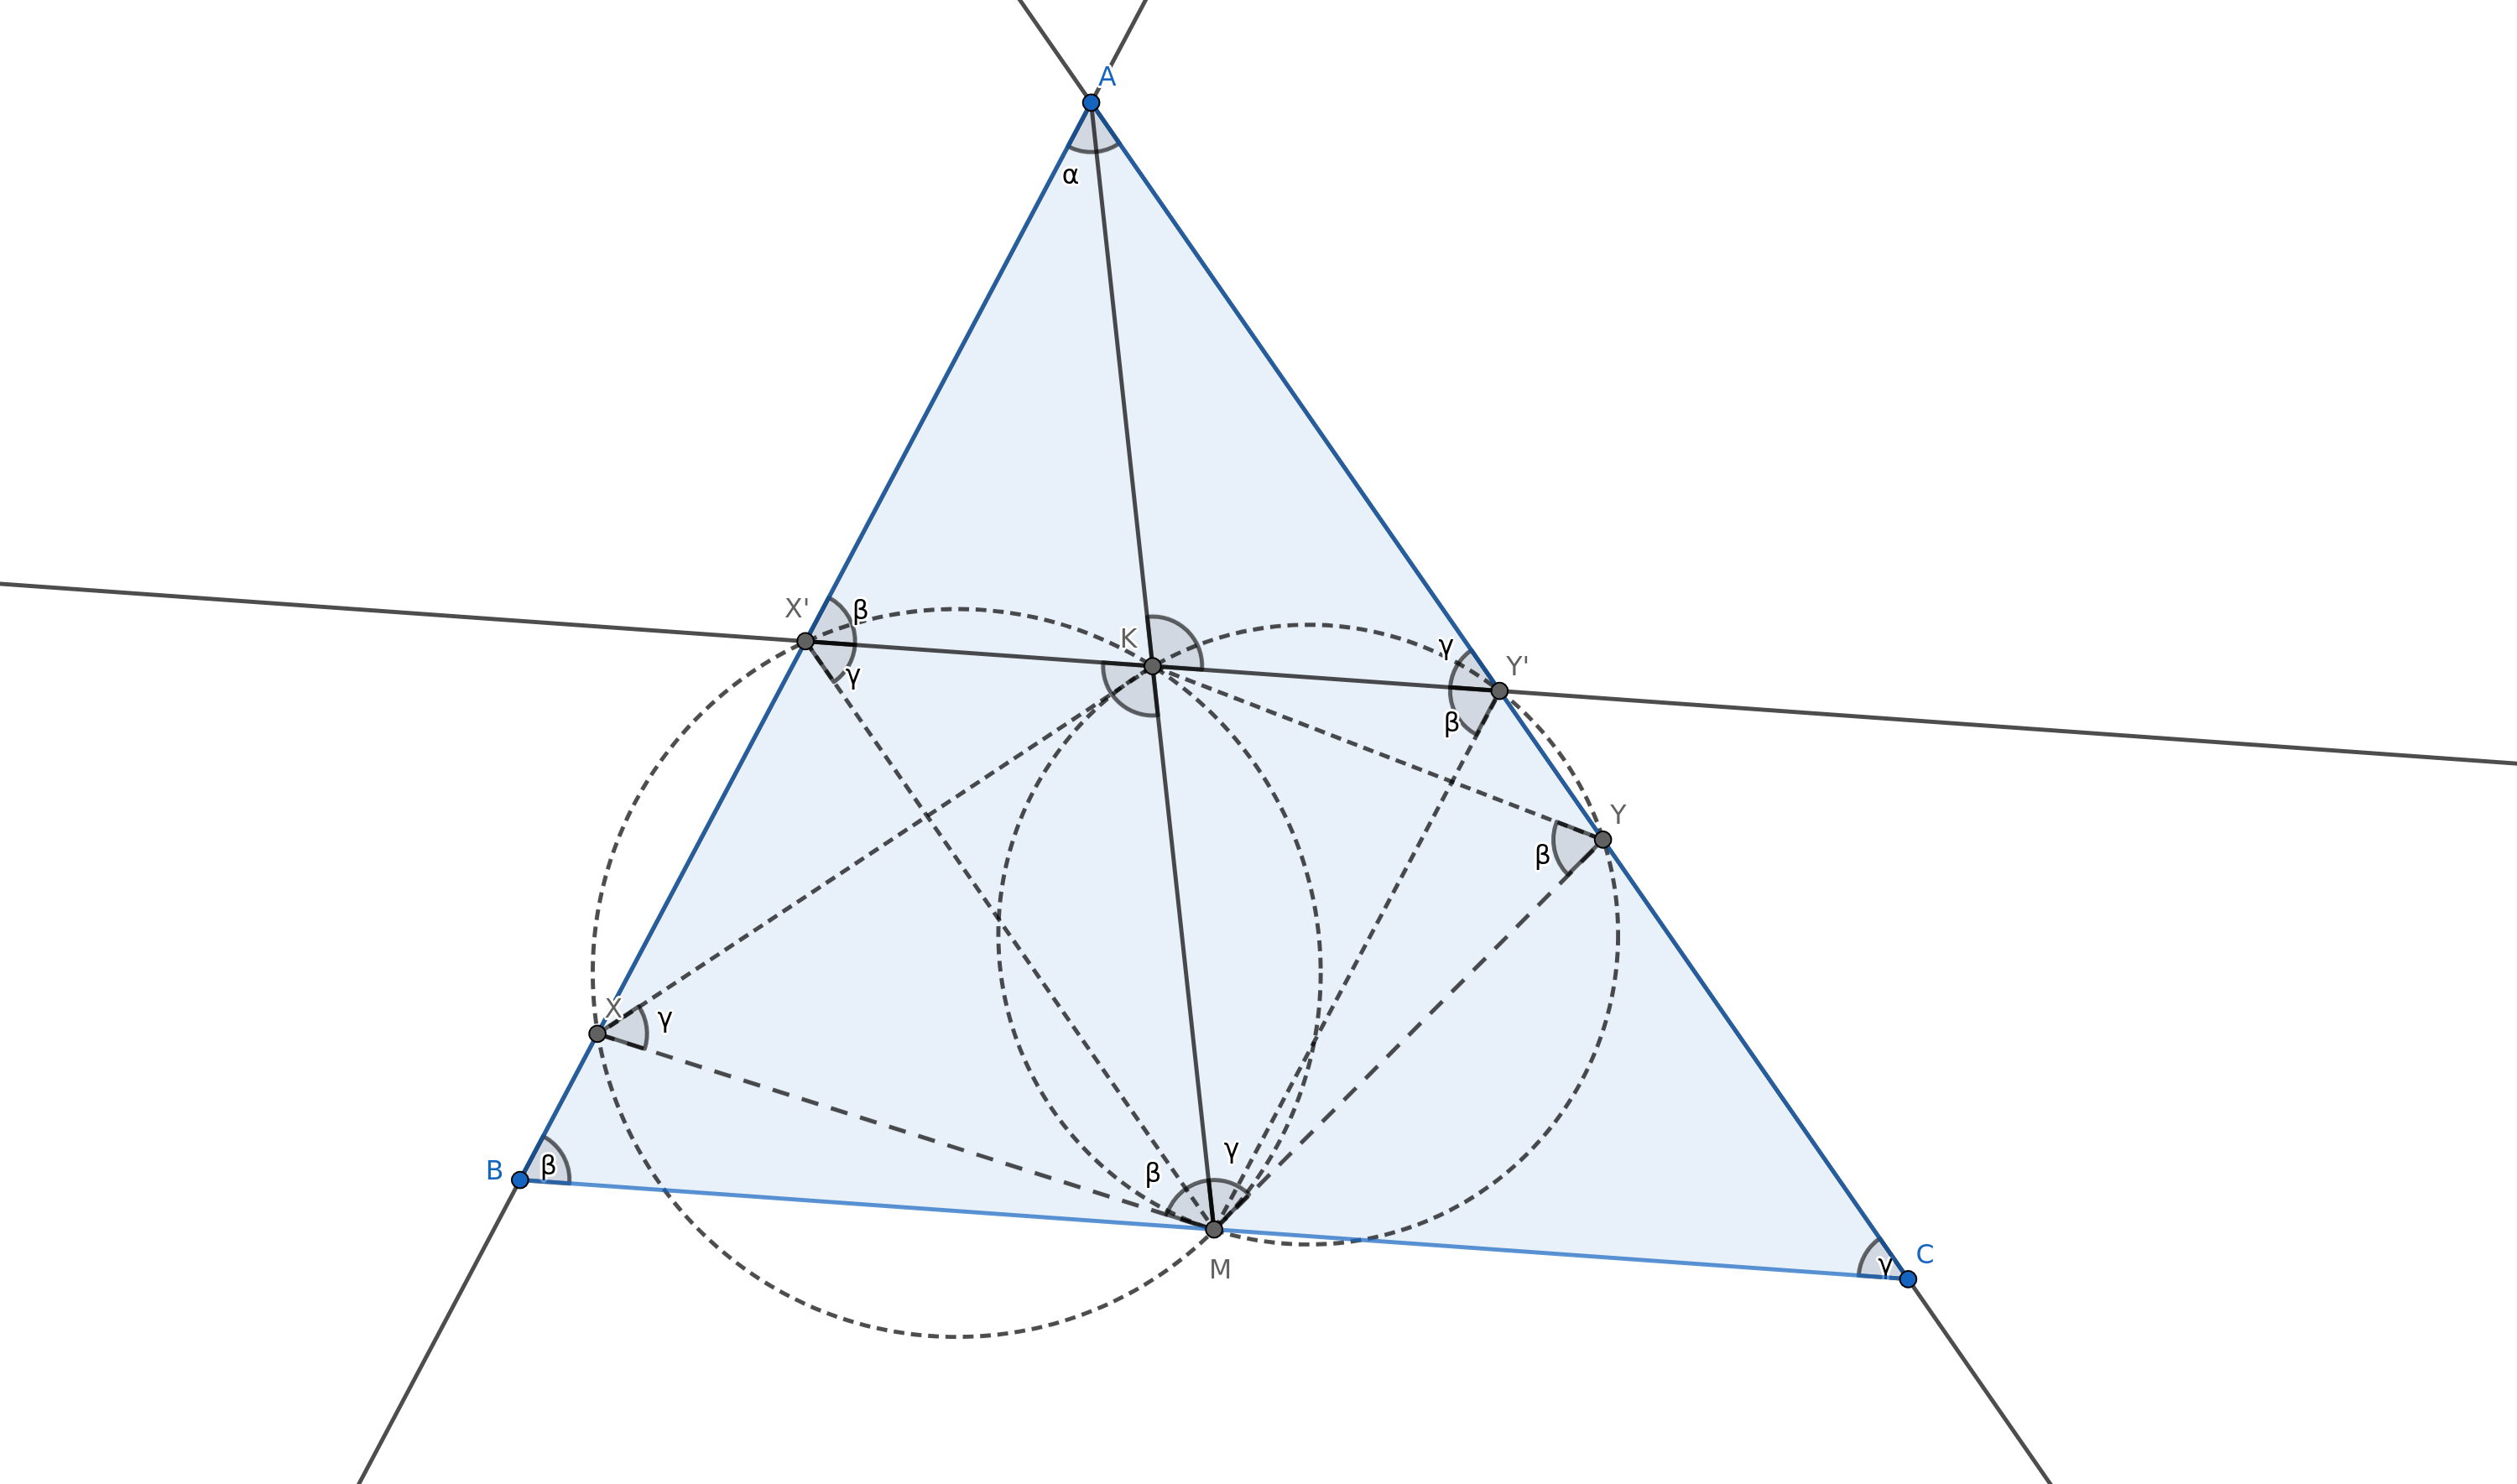
\includegraphics[width=0.95\textwidth]{G-fig.png}
  \end{center}
  \caption{Konstrukce úlohy}
  \label{fig:1}
\end{figure}


Nechť body $X'$ a $Y'$ jsou středy stran $AB$ a $AC$. Jako první dokážeme shodnost trojúhelníků $AY'K$ a $MX'K$. Protože body $X'$, $K$ a $Y'$ leží na střední příčce, úhly při vrcholu $K$ jsou shodné a bod $K$ půlí jak úsečku $AM$, tak úsečku $X'Y'$, z čehož nutně plyne shodnost trojúhelníků $AY'K$ a $MX'K$. Podobně ukážeme i shodnost trojúhelníků $AKX'$ a $MKY'$.

Ze shodnosti těchto trojúhelníků platí rovnosti $|\angle KX'M| = |\angle KXM| = |\angle ACB| = \gamma$ a $|\angle KY'M| = |\angle KYM| = |\angle ABC| = \beta$, proto jsou čtyřúhelníky $KMXX'$ a $Y'YMK$ tětivové. Úhlením pak přijdeme na rovnost $|\angle AMX| = \beta$ a $|\angle AMY| = \gamma$ (viz konstrukce na obrázku \ref{fig:1}). Pak podle věty uu platí podobnosti $ABM \sim AMX$ a $AMC \sim AYM$.

Teď už umíme ukázat, že body $B$, $C$, $X$, $Y$ leží na kružnici, a to pomocí rovnice vycházející z mocnosti bodu ke kružnici:

\begin{equation} \label{eq:1}
  |AX| \cdot |AB| = |AY| \cdot |AC|
\end{equation}

Z podobnosti trojúhelníků $ABM \sim AMX$ platí:
\[
  \frac{|AB|}{|AM|} = \frac{|AM|}{|AX|} \ztoho |AM|^2 = |AX| \cdot |AB|
\]

A z podobnosti trojúhelníků $AMC \sim AYM$ platí:

\[
  \frac{|AC|}{|AM|} = \frac{|AM|}{|AY|} \ztoho |AM|^2 = |AY| \cdot |AC|
\]

Rovnice \ref{eq:1} tedy zřejmě platí, proto body $B$, $C$, $X$, $Y$ leží na kružnici, jak jsme chtěli dokázat.


\end{document}

